\chapter{Další možné využití}

%Původní nápad -- proč je použit ohebný pásek? 		
Můj původní nápad byl, že mojí ročníkovou prací bude výroba plnohodnotné Lampičky, počítaje jak elektrotechnickou část tak tu Designovou. Z toho boužel sešlo z časových důvodů a tak tu teoreticky proberu Designovou část. 
Důvod proč jsem později zaměnila pevní LED pásek za ohebný, byl ten, že původně jsem měla nápad na to, že Ty ohebné LED by se dali lépe vsunout do předem připravené plasové žárovky. Žárovka by byla tvořená z průhledné Křišťálové pryskyřice tzv. Epoxy resinu což je čirá odlívací tekutina používající se jak na umělecké, tak technícké účely. Z toho sešlo kvůli problémům zvládnutí této techniky a nedostatku času. %todo reference a odkaz na pryskyřici

%Další nápady -- Více světel bez/drátově propojená. 		
Šlo by také vytvořit více ESP32-DevkitC s LED, které by byli navzájem propojené, ať už bezdrátově, nebo dráty. V bezdrátové verzi vidím víc výhod, ale zase by mohl být problém s dosahem a dálkou od ovládacího zařízení. 
Na více světel by se dalo vyrobit více tzv. žárovek tím, že by se podle předem vytvořeného originálu vyrobila forma na silikon a ta by se následně opakovaně použila na odlití Epoxidové priskyřice. Každá ze světel by měla tzv. "základnu", která by byla buď vytvořená z dřevěných desek přesně vypálených na laseru, a nebo by se na to dal vytisknout plastový obal na 3D tiskárně, což je možnost, která se mi líbí víc. 
	
%todo tzv základna a žárovka oznažit kurzívou? 
%todo laser odkaz??? 3d tiskárna odkaz?		

S trochou snahy, kreativity a hodně práce by se z tohoto prototypu mohla stát i sada pro "začínající" programátory a elektroniky, protože to pokryje jak pájení a práci s elektronickými součástkami, tak programování kdy člověk muže buď už předem naprogramovaný program stáhnout z internetu, nebo si ho naprogramovat a upravit podle sebe Obávám se ale že s tímto nápadem by byli menší problémy, protože celkově jak knihovny, tak aplikace, původní program a návod jak s tím pracovat vznikl v rámci Letního Robotického tábora který pořádá každý rok Helceltka, a tím pádem by mohl nastat problém ohledně plagiátorství nápadu 

%todo reference na aplikaci rbcontrol; původní program; Robotický tábor

Ráda bych tuto ročníkovou práci ukončila s myšlenkou, že můj protoryp svítících LED světel má kreativní využití ve všech směrech a je jen na konstruktérovi, jak bude tento nápad chtít využít. 


%   \begin{figure}[htbp]
%	\centering
%	\begin{minipage}[b]{0.5\textwidth}
%		\centering
%		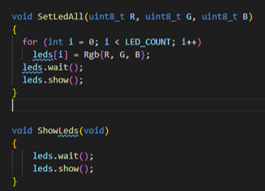
\includegraphics[width=0.75\textwidth]{img/015 img/definovane-funkce.png}
%		\caption{Funkce}
%		%		\label{fig:gear-sketch1}
%	\end{minipage}
%	\qquad
%	\begin{minipage}[b]{0.4\textwidth}
%		\centering
%		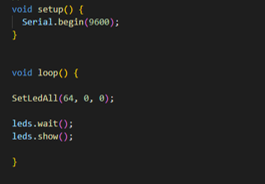
\includegraphics[width=1\textwidth]{img/015 img/Program1-červená.png}
%		\caption{Program}
%		%		\label{fig:gear-sketch2}
%	\end{minipage}
%\end{figure}

\newpage